\documentclass[12pt,a4paper,fontset=none]{ctexart}
\usepackage{ctex}
\usepackage{emptypage} 
\usepackage{fancyhdr}
\usepackage{amsmath,amsfonts,amssymb,mathtools}
\usepackage{graphicx}
\usepackage{mathptmx}
\usepackage{booktabs}
\usepackage[labelfont=bf]{caption}
\usepackage{indentfirst}
\usepackage{caption}
\usepackage{enumitem}
\usepackage[marginal]{footmisc}
\usepackage{subfigure}
\usepackage{fontspec}
\usepackage{geometry}
\usepackage{setspace}
\usepackage{listings}
\usepackage{xcolor}
\usepackage{float}
\usepackage{pifont}
\usepackage{algorithm}
\usepackage{algorithmic}
\newgeometry{left=3cm,top=2.5cm,bottom=2.5cm,right=3cm}
\setmainfont{Times New Roman}
\setCJKmainfont[BoldFont=SimHei,ItalicFont=KaiTi]{SimSun}

\lstset{
	backgroundcolor=\color{green!10!blue!15},
	rulesepcolor= \color{red!40!blue!100},
	breaklines=true,
	breakatwhitespace=false,
	numbers=left, 
	numberstyle= \small,
	keywordstyle= \color{blue},
	commentstyle=\color{gray}, 
	frame=shadowbox
}

\renewcommand{\baselinestretch}{1.5}

\title{\textbf{概率论与数理统计第四次作业}}

\author{
\\
\Large{麻超 \quad 201300066}
\\[6pt]
{ \large \textit{南京大学人工智能学院}}\\[2pt]
}

\date{\today}
\newcommand{\supercite}[1]{\textsuperscript{\cite{#1}}}

\begin{document}
\maketitle
\setcounter{page}{1}

\section*{3.1}
证明:由二项分布的定义,P(X=k)表示n重伯努利实验中A发生的次数,故$P(X)=\binom{n}{k}p^k(1-p)^{n-k}$,故
\begin{align*}
	E(x) & =\sum_{k=0}^nk\binom{n}{k}p^k(1-p)^{n-k}           \\
	E(x) & =(1-p)^n\sum_{k=1}^n\binom{n}{k}k(\frac{p}{1-p})^k
\end{align*}
由二项展开式
\begin{align*}
	(1+x)^n=\sum_{k=0}^n\binom{n}{k}kx^{n-1}
\end{align*}
两边同求导数,得
\begin{align*}
	n(1+x)^{n-1}  & =\sum_{k=1}^n\binom{n}{k}kx^{k-1} \\
	nx(1+x)^{n-1} & =\sum_{k=1}^n\binom{n}{k}kx^k
\end{align*}
由于x=p/(1-p),故代入可得
\begin{align*}
	E(x)=(1-p)^n\sum_{k=1}^n\binom{n}{k}k(\frac{p}{1-p})^k=(1-p)^n\frac{np}{(1-p)^n}=np
\end{align*}
对于方差,有:
\begin{align*}
	D(x)   & =E(X^2)-E(X)^2                             \\
	E(X^2) & =\sum_{k=0}^nk^2\binom{n}{k}p^k(1-p)^{n-k}
	\\ &=\sum_{k=1}^nk(k-1)\binom{n}{k}p^k(1-p)^{n-k}+np
	\\ &=(1-p)^n\sum_{k=2}^nk(k-1)\binom{n}{k}\frac{p}{1-p}^k+np
\end{align*}
对上方二项展开式$(1+x)^n=\sum_{k=0}^n\binom{n}{k}x^k$求导两次可得,
\begin{align*}
	n(n-1)(1+x)^{n-2}    & =\sum_{k=2}^n\binom{n}{k}k(k-1)x^{k-2} \\
	n(n-1)(1+x)^{n-2}x^2 & =\sum_{k=2}^n\binom{n}{k}k(k-1)x^k
\end{align*}
代入x=p/(1-p)可得:
\begin{align*}
	E(x^2) & =n(n-1)p^2+np=n^2p^2+np(1-p) \\
	E(X)^2 & =n^2p^2
\end{align*}
$\therefore Var(X)=E(X^2)-E(X)^2=np(1-p)$.
\section*{3.2}
由几何分布的定义,几何分布X~G(p)得分布列为$P(X=k)=(1-p)^{k-1}p$

故对几何分布有:
\begin{align*}
	E(X)=\sum_{k=1}^\infty kp(1-p)^{k-1}=p\sum_{k=1}^\infty k(1-p)^k-1
\end{align*}
对级数展开式$(1-x)^{-1}=\sum_{k=0}^\infty x^k$两边求导有:
\begin{align*}
	\sum_{k=1}^\infty kx^{k-1} & =\frac{1}{(1-x)^2}
\end{align*}
令x=1-p,有:
\begin{align*}
	E(X)=p\frac{1}{(1-(1-p))^2} & =\frac{1}{p}
\end{align*}
对于方差,有:
\begin{align*}
	E(X^2)=\sum_{k=1}^{\infty}k^2p(1-p)^{k-1}=p\sum_{k=2}^{\infty}k(k-1)(1-p)^{k-1}+1/p
\end{align*}
对级数展开式$(1-x)^{-1}=\sum_{k=0}^\infty x^k$两边求二阶导得:
\begin{align*}
	\sum_{k=}^{\infty}k(k-1)x^{k-2}=\frac{2}{(1-x)^3} \\
	\sum_{k=}^{\infty}k(k-1)x^{k-1}=\frac{2x}{(1-x)^3}
\end{align*}
令x=1-p得,$E(X^2)=(2-p)/p^2$\dots
\begin{align*}
	\therefore Var(X)=E(X^2)-E(X)^2=(2-p)/p^2-1/p^2=(1-p)/p^2
\end{align*}
\section*{3.3}
对于负二项分布,有$P(X=k)=\binom{k-1}{r-1}p^{r-1}(1-p)^{k-r}p=\binom{k-1}{r-1}p^r(1-p)^{k-r},k=r,r+1...$

故对于期望E(X)有:
\begin{align*}
	E(X) & =\sum_{k=r}^{\infty}k\binom{k-1}{r-1}p^r(1-p)^{k-r}           \\
	     & =\frac{r}{p}\sum_{k=r}^{\infty}\binom{k}{r}p^{r+1}(1-p)^{k-r}
\end{align*}
由于\begin{align*}
	\sum_{k=r}^{\infty}\binom{k+1-1}{r+1-1}p^{r+1}(1-p)^{k-r}=1.
\end{align*}
故\begin{align*}
	E(X)=\frac{r}{p}
\end{align*}
对于方差的计算,类似地有:
\begin{align*}
	E(X^2) & =\sum_{k=r}^{\infty}\binom{k-1}{r-1}p^r(1-p)^{k-r}                                                                                \\
	       & =\frac{r}{p}\sum_{k=r}^{\infty}(k+1-1)\binom{k}{r}p^r(1-p)^{k-r}                                                                  \\
	       & =\frac{r(r+1)}{p^2}\sum_{k=r}^{\infty}\binom{k+1}{r+1}p^{r+1}(1-p)^{k-r}-\frac{r}{p}\sum_{k=r}^{\infty}\binom{k}{r}p^r(1-p)^{k-r} \\
	       & =\frac{r(r+1)}{p^2}-\frac{r}{p}
\end{align*}
所以可以得到
\begin{align*}
	Var(X)=E(X^2)-E(X)^2=\frac{r(r+1)}{p^2}-\frac{r}{p}-\frac{r^2}{p^2}=\frac{r(1-p)}{p^2}
\end{align*}
\section*{3.4}

对于泊松分布有:P(X=k)=$\frac{\lambda ^k}{k!}e^{-\lambda},(k=0,1,2...) $
所以对于期望有:
\begin{align*}
	E(X)=\sum_{k=1}^{\infty}k\frac{\lambda^k}{k!}e^{-\lambda}=\lambda e^{-\lambda}\sum_{k=1}^{\infty} \frac{\lambda ^{k-1}}{(k-1)!}
\end{align*}
由于泰勒展开式$e^x=1+x+\frac{x^2}{2!}+...=\sum_{k=1}^{\infty}\frac{x^{k-1}}{(k-1)!}  $
所以其期望为
\begin{align*}
	E(X)=\lambda e^{-\lambda}e^{\lambda}=\lambda
\end{align*}
对于方差,有:\begin{align*}
	E(X^2) & =\sum_{k=0}^{\infty}k^2\frac{\lambda ^k}{k!}e^{-\lambda}                       \\&=\lambda e^{-\lambda}\sum_{k=1}^{\infty} \frac{k\lambda ^{k-1}}{(k-1)!}\\
	       & = \lambda e^{-\lambda}\sum_{k=1}^{\infty} \frac{(k-1+1)\lambda ^{k-1}}{(k-1)!}
\end{align*}
令m=k-1,则有:\begin{align*}
	E(X^2) & =\lambda e^{-\lambda}(\sum_{m=0}^{\infty} \frac{m\lambda ^{m}}{m!}+\sum_{m=0}^{\infty}\frac{\lambda ^m}{m!} )             \\
	       & =\lambda e^{-\lambda}(\lambda \sum_{m=1}^{\infty}\frac{\lambda ^{m-1}}{(m-1)!}+\sum_{m=0}^{\infty}\frac{\lambda ^m}{m!} ) \\
	       & =\lambda e^{-\lambda}(\lambda e^{\lambda}+e^{\lambda})                                                                    \\ &=\lambda(\lambda+1)
\end{align*}
故计算得方差\begin{align*}
	D(X)=E(X^2)-E(X)^2=\lambda(\lambda+1)-\lambda^2=\lambda
\end{align*}
\section*{3.5}
用H表示某个叶节点的高度,设$X_i$表示第i轮中该叶节点是否被选中,选中时有$X_i=1$,否则其等于0.

在第i轮时一共有i个节点,故该节点选中的概率$P(X_i=1)=\frac{1}{i} $.

则$E(X_i)=1\cdot P(X_i=1)=\frac{1}{i} $

所以有$E(H)=E(\sum_{i=1}^{k}X_i)=\sum_{i=1}^{k}=\sum_{i=1}^{k}\approx O(\ln k)$
\section*{3.6}
\subsection*{1}
在有放回的情况下,X可能的取值一共有1到10,共10种可能性.
其中P(1)=$\frac{1}{10^5} $,而P(2)=($(\frac{2}{10})^5$-P(1))=$\frac{31}{10^5} $
分布列如下:
\begin{center}
	\begin{tabular}{|c|c|c|c|c|c|c|c|c|c|c|}
		\hline
		X    & 1                 & 2                  & 3                   & 4                   & 5                    & 6                    & 7                    & 8                     & 9                     & 10                    \\
		\hline
		P(X) & $\frac{1}{10^5} $ & $\frac{31}{10^5} $ & $\frac{211}{10^5} $ & $\frac{781}{10^5} $ & $\frac{2101}{10^5} $ & $\frac{4651}{10^5} $ & $\frac{9031}{10^5} $ & $\frac{15961}{10^5} $ & $\frac{26281}{10^5} $ & $\frac{40951}{10^5} $ \\
		\hline
	\end{tabular}
\end{center}

在无放回情况下,X可能取值为5,6,7,8,9,10.总情况为$\binom{10}{5}=252$.对于X=5来说,只有一种情况,故P(X=5)=$\frac{1}{252} $,其他情况类似.分布列如下:

\begin{center}
	\begin{tabular}{|c|c|c|c|c|c|c|}
		\hline
		X    & 5                & 6                & 7                 & 8                 & 9                 & 10                 \\
		\hline
		P(X) & $\frac{1}{252} $ & $\frac{5}{252} $ & $\frac{15}{252} $ & $\frac{35}{252} $ & $\frac{70}{252} $ & $\frac{126}{252} $ \\
		\hline
	\end{tabular}
\end{center}

\section*{3.7}
由题意,这种情况下,令M表示在这100+x个元件中不合格元件数,即M服从n=100+x和p=0.01的二项分布,记事件A为至少有100个合格零件,则$P(A)=\sum_{k=1}^{x}\binom{100+x}{k}(0.01)^k(0.99)^{100+x-k}$.

利用泊松定理近似模拟,得到P(A)=$\sum_{k=1}^{x}\frac{e^{-1}}{k!} $

当x=0,1,2,3时,上式中P(A)分别等于0.368,0.736,0.920,0.981.故x的最小值为3.

\section*{3.8}
\subsection*{3.8.2}
这道题和3.6.2类似,直接写出分布列:

\begin{center}
	\begin{tabular}{|c|c|c|c|c|c|c|}
		\hline
		X    & 3               & 4               & 5               \\
		\hline
		P(X) & $\frac{1}{10} $ & $\frac{3}{10} $ & $\frac{6}{10} $ \\
		\hline
	\end{tabular}
\end{center}
\subsection*{3.8.3}
X所有可能的取值为0,1,2.其中,由于为不放回抽样,故求得概率:

\begin{align*}
	P(X=0) & =\binom{13}{3}/\binom{15}{3}=\frac{286}{455}             \\
	P(X=1) & =\binom{13}{2}\binom{2}{1}/\binom{15}{3}=\frac{156}{455} \\
	P(X=2) & =\binom{13}{1}\binom{2}{2}/\binom{15}{3}=\frac{13}{455}
\end{align*}

分布列如下:

\begin{center}
	\begin{tabular}{|c|c|c|c|}
		\hline
		X    & 0                  & 1                  & 2                 \\
		\hline
		P(X) & $\frac{286}{455} $ & $\frac{156}{455} $ & $\frac{13}{455} $ \\
		\hline
	\end{tabular}
\end{center}

\begin{figure}[H]
	\centering
	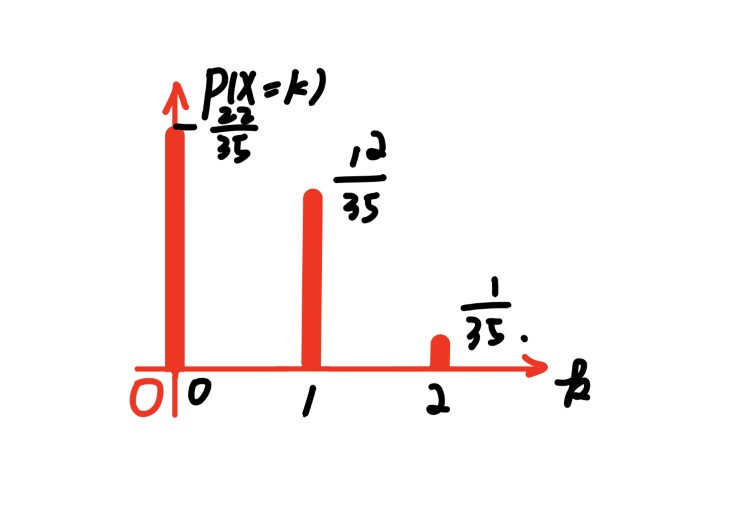
\includegraphics[width=0.7\linewidth]{习题图.jpg}
	\caption{3.8.3附图}
\end{figure}
\section*{3.9}
\subsection*{3.9.2}
首先求检验一次决定需要调整设备的概率,记为p.

设每次抽检次品数量为X,则X$\sim $b(10,0.1).则有:

\begin{align*}
	p=P(Y>1)=1-P(Y=0)-P(Y=1)=1-0.9^{10}-\binom{10}{1}\cdot 0.9^9\cdot 0.1=0.264
\end{align*}

又因为每一次实验结果相互独立,于是有

\begin{align*}
	X\sim b(4,0.264)
\end{align*}

于是有

\begin{align*}
	E(X)=np=1.056
\end{align*}

\subsection*{3.9.3}
易知共有$4^3=64$种可能性,X的所有可能的取值为1,2,3,4.

3只球都放在4号盒子的放法只有1种,故$P(X=4)=\frac{1}{64} $

X=3表示1,2号盒子是空的,球都在3,4号盒子里面放,共有$2^3=8$种放法,但其中一种与X=4重复,故只有7种.即$P(X=3)=\frac{7}{64} $

同理,$P(X=2)=\frac{19}{64},P(X=1)\frac{37}{64}  $.

于是有:

\begin{align*}
	E(X)=1\times \frac{37}{64} +2\times \frac{19}{64} +3\times \frac{7}{64}+4\times \frac{1}{64} =\frac{25}{16}.
\end{align*}

\section*{3.10}
\subsection*{3.10.4}
\subsubsection*{(1)}
因为级数

\begin{align*}
	\sum_{j=1}^{\infty} & (-1)^{j+1}\frac{3^j}{j}P(X=(-1)^{j+1}\frac{3^j}{j} )          \\
	=                   & \sum_{j=1}^{\infty}(-1)^{j+1}\frac{3^j}{j}\cdot \frac{2}{3^j}
	=                   & 2\sum_{j=1}^{\infty}\frac{(-1)^{j+1}}{j}
\end{align*}

不是一个绝对收敛的级数,故按照定义可知其数学期望不存在.

\subsubsection*{(2)}
记$A_k$表示第k次摸到了黑球,同时记$\overline{A_k}$表示第k次摸到了白球.以$B_k$表示游戏在第k次结束,由题意可知:

$C_k=A_1A_2...A_{k-1}\overline{A_k}$\\
$P(C_k)=P(\overline{A_k}|A_1A_2...A_{k-1})P(A_{k-1}|A_1A_2...A_{k-2})...P(A_2|A_1)P(A_1)$.

于是由定义:

$P(X=1)=P(\overline{A_1})=\frac{1}{2} $\\
$P(X=2)=P(\overline{A_2}|A_1)P(A_1)=\frac{1}{6} $\\
$P(X=3)=P(\overline{A_3}|A_2A_1)P(\overline{A_2}|A_1)P(A_1)=\frac{1}{12} $\\
故

\begin{align*}
	P(X=k) & =P(\overline{A_k}|A_1A_2...A_{k-1})P(A_{k-1}|A_1A_2...A_{k-2})...P(A_2|A_1)P(A_1) \\
	       & =\frac{1}{k+1}\frac{k-1}{k}\frac{k-2}{k-1}...\frac{2}{3}\frac{1}{2}               \\
	       & =\frac{1}{k(k+1)}
\end{align*}

但是

\begin{align*}
	\sum_{k=1}^{\infty}kP(X=k)=\sum_{k=1}^{\infty}k\frac{1}{k+1}\frac{1}{k}=\sum_{k=1}^{\infty}\frac{1}{k+1}=\infty
\end{align*}

故E(X)不存在.
\subsection*{3.10.6}
\subsubsection*{(1)}
\begin{align*}
	E(X)      & =(-2)\times 0.4+0+2\times 0.3=-0.2    \\
	E(X^2)    & =(-2)^2\times 0.4+0+2^2\times 0.3=2.8 \\
	E(3X^2+5) & =3E(X^2)+5=8.4+5=13.4
\end{align*}

\subsubsection*{(2)}
由于$X\sim \pi(\lambda)$,故$P(X=k)=\frac{\lambda^ke^{-\lambda}}{k!} $

所以有:
\begin{align*}
	E(\frac{1}{X+1} ) & =\sum_{k=0}^{\infty}\frac{1}{k+1}P(X=k)                                      \\
	                  & =\sum_{k=0}^{\infty}\frac{1}{k+1} \frac{\lambda^ke^{-\lambda}}{k!}           \\
	                  & =\frac{e^{-\lambda}}{\lambda}\sum_{k=0}^{\infty}\frac{\lambda^{k+1}}{(k+1)!} \\
	                  & =\frac{e^{-\lambda}}{\lambda}(e^{\lambda}-1)                                 \\
	                  & =\frac{1}{\lambda}(1-e^{-\lambda}).
\end{align*}
\end{document}